\documentclass[12pt,a4paper,openany]{book}
\usepackage{lmodern}
\usepackage[svgnames]{xcolor} % Required to specify font color
\input{/home/aroquemaurel/cours/includesLaTeX/couleurs.tex}

\usepackage[utf8]{inputenc} 
\usepackage[T1]{fontenc}
\usepackage[francais]{babel}
\usepackage[top=1.7cm, bottom=1.7cm, left=1.7cm, right=1.7cm]{geometry}
\usepackage{verbatim}
\usepackage[urlbordercolor={1 1 1}, linkbordercolor={1 1 1}, linkcolor=vert1, urlcolor=bleu, colorlinks=true]{hyperref}
\usepackage{tikz} %Vectoriel
\usepackage{listings}
\usepackage{fancyhdr}
\usepackage{multido}
\usepackage{amssymb}
\usepackage{float}
\usepackage[francais]{minitoc}
\usepackage[final]{pdfpages} 
\usepackage{graphicx} % Required for box manipulation

\newcommand{\titre}{Base de données}
\newcommand{\subtitle}{SQL}
\newcommand{\auteur}{Antoine de \bsc{Roquemaurel}}
\newcommand{\formation}{L3 Informatique}
\newcommand{\semestre}{5}
\newcommand{\annee}{2013}
\newcommand{\prof}{~}


\newcommand{\pole}{}
\newcommand{\sigle}{bdd}


\input{/home/aroquemaurel/cours/includesLaTeX/listings.tex}
\documentclass[12pt,a4paper,openany]{book}
\usepackage{lmodern}
\usepackage{xcolor}
\input{/home/aroquemaurel/cours/includesLaTeX/couleurs.tex}

\usepackage[utf8]{inputenc}
\usepackage[T1]{fontenc}
\usepackage[francais]{babel}
\usepackage[top=1.7cm, bottom=1.7cm, left=1.7cm, right=1.7cm]{geometry}
\usepackage{verbatim}
\usepackage[urlbordercolor={1 1 1}, linkbordercolor={1 1 1}, linkcolor=vert1, urlcolor=bleu, colorlinks=true]{hyperref}
\usepackage{tikz} %Vectoriel
\usepackage{listings}
\usepackage{fancyhdr}
\usepackage{multido}
\usepackage{amssymb}
\usepackage{float}
\usepackage[francais]{minitoc}

\newcommand{\titre}{Complexité des algorithmes}

\newcommand{\pole}{}
\newcommand{\sigle}{complexite}

\newcommand{\semestre}{3}

\input{/home/aroquemaurel/cours/includesLaTeX/listings.tex} %prise en charge du langage C 
\input{/home/aroquemaurel/cours/includesLaTeX/entete-l2-cours.tex}




%----------------------------------------------------------------------------------------
%	DEFINITION OF COLORED BOXES
%----------------------------------------------------------------------------------------

\RequirePackage[framemethod=default]{mdframed} % Required for creating the theorem, definition, exercise and corollary boxes

% Theorem box
\newmdenv[skipabove=7pt,
skipbelow=7pt,
backgroundcolor=black!5,
linecolor=ocre,
innerleftmargin=5pt,
innerrightmargin=5pt,
innertopmargin=5pt,
leftmargin=0cm,
rightmargin=0cm,
innerbottommargin=5pt]{tBox}

% Exercise box	  
\newmdenv[skipabove=7pt,
skipbelow=7pt,
rightline=false,
leftline=true,
topline=false,
bottomline=false,
backgroundcolor=ocre!10,
linecolor=ocre,
innerleftmargin=5pt,
innerrightmargin=5pt,
innertopmargin=5pt,
innerbottommargin=5pt,
leftmargin=0cm,
rightmargin=0cm,
linewidth=4pt]{eBox}	

% Definition box
\newmdenv[skipabove=10pt,
skipbelow=10pt,
rightline=false,
leftline=true,
topline=false,
bottomline=false,
linecolor=ocre,
innerleftmargin=5pt,
innerrightmargin=5pt,
innertopmargin=0pt,
leftmargin=0cm,
rightmargin=0cm,
linewidth=4pt,
innerbottommargin=0pt]{dBox}	

% Corollary box
\newmdenv[skipabove=7pt,
skipbelow=7pt,
rightline=false,
leftline=true,
topline=false,
bottomline=false,
linecolor=gray,
backgroundcolor=black!5,
innerleftmargin=5pt,
innerrightmargin=5pt,
innertopmargin=5pt,
leftmargin=0cm,
rightmargin=0cm,
linewidth=4pt,
innerbottommargin=5pt]{cBox}		

% Corollary box
\newmdenv[skipabove=7pt,
skipbelow=7pt,
rightline=true,
leftline=false,
topline=false,
bottomline=true,
linecolor=gray,
backgroundcolor=black!5,
innerleftmargin=5pt,
innerrightmargin=5pt,
innertopmargin=5pt,
leftmargin=0cm,
rightmargin=0cm,
linewidth=1pt,
innerbottommargin=5pt]{rBox}				  
		  

% Creates an environment for each type of theorem and assigns it a theorem text style from the "Theorem Styles" section above and a colored box from above
\newenvironment{theorem}{\begin{tBox}\begin{theoremeT}}{\end{theoremeT}\end{tBox}}
\newenvironment{example}{\begin{exampleT}}{\hfill{\tiny\ensuremath{\blacksquare}}\end{exampleT}}
\newenvironment{definition}{\begin{dBox}\begin{definitionT}}{\end{definitionT}\end{dBox}}
\newenvironment{attention}{\begin{eBox}\small}{\end{eBox}}				  	
\newenvironment{exemple}{\begin{cBox}\small}{\end{cBox}}	

%----------------------------------------------------------------------------------------
%	REMARK ENVIRONMENT
%----------------------------------------------------------------------------------------

\newenvironment{remarque}{\par\vskip10pt\small
\begin{rBox}
\begin{list}{}{
\leftmargin=35pt % Indentation on the left
\rightmargin=25pt}\item\ignorespaces % Indentation on the right
\makebox[-2.5pt]{\begin{tikzpicture}[overlay]
\node[draw=ocre!60,line width=1pt,circle,fill=ocre!25,font=\sffamily\bfseries,inner sep=2pt,outer sep=0pt] at (-15pt,0pt){\textcolor{ocre}{R}};\end{tikzpicture}} % Orange R in a circle
\advance\baselineskip -1pt}
{\end{list}\vskip1mm\end{rBox}\vskip5pt} % Tighter line spacing and white space after remark



\input{/home/aroquemaurel/cours/includesLaTeX/polices.tex}
\input{/home/aroquemaurel/cours/includesLaTeX/affichageChapitre.tex}
\newcommand{\pfp}{\texttt{pfp}}

\newcommand{\ifp}{\texttt{if}}
\newcommand{\moy}{\textrm{moy}}
\newcommand{\prob}{\textrm{prob}}
\newcommand{\elsep}{\texttt{else}}
\newcommand{\perm}{\texttt{perm}}
\newcommand{\random}{\texttt{perm}}

\makeatother
\includeonly{
chapitre1,
chapitre2,
chapitre3,
%chapitre4,
annexes,
}
\begin{document}
	\frontmatter
	\setcounter{tocdepth}{1}
	\setcounter{secnumdepth}{3}
	\setcounter{minitocdepth}{1}
	\dominitoc
	\maketitle
	\chapter*{Modalité de Contrôle de connaissance}
	\begin{enumerate}
		\item Devoir Maison à rendre avant 10h le 21 décembre. (10\%)
		\item Contrôle de continue sous forme de QCM lundi 3 décembre de 8h15 à 9h45 (20\%)
		\item Contrôle terminal vendredi 21 décembre de 10h à 12h (70\%)
	\end{enumerate}
	\tableofcontents
	\mainmatter
	\chapter{Projet et Équipe de management}
	\section{Présentation des créateurs}
		\begin{itemize}
			\item \Bonte{}, Ingénieur en \gHabitat{}
			\item \Ben{}, Ingénieur en \gHabitat{}
			\item \Drm{}, Développeur Web
			\item \Soum{}, Développeur \texttt{\glo{C++}{C++}{4e langage de programmation
				le plus utilisé au monde. Il est compilé, permettant de produire un programme
				s'éxecutant le plus rapidement possible.}/\glo{Qt}{Qt}{Bibliothèque programmée
				en C++ permettant de créer des interfaces graphiques.}}
			\item \Clem{}, Développeur \texttt{C++/Qt}, Administrateur Système et Réseau
		\end{itemize}
		
		\subsection{Formations}
			\Bonte{} et \Ben{} ont obtenu un Master Pro \gHabitat{} à l'INSA de Toulouse et
			font actuellement une thèse.

			\Drm{}, \Soum{} et \Clem{} sont en deuxième année de DUT Informatique 
			à l'IUT Paul Sabatier de Toulouse. Ces derniers sont
			également autodidactes et ont pu acquérir de nombreuses conpétences lors de projets personnels.
	
		\subsection{Expériences professionnelles}
			\Bonte{} a passé un an dans un bureau d'étude à réaliser des bilans thermique. C'est pendant cette periode 
			que lui est venue l'idée de notre projet après avoir constaté le manque dramatique d'affordance des solutions disponibles.
			Le reste de l'équipe s'est constitué autour de ce constat global.
	
	\section{Atouts}
		%atouts qui font qu'on a des facilités a créer l'entreprise

		%facultés particulières
		Ayant déja eu une expérience professionnelle, \bonte{} et \ben{} connaissent les difficultés et les besoins des TPE et PME du \gHabitat{}.
		%contacts
		Ainsi, nous disposons déja de contacts dans ce secteur,
		nottamment au sein d'établissements universitaires et de bureaux d'étude.
		Ce premier carnet d'adresse peut être facilement étoffé car notre clientelle est,
		par sa taille humaine, facilement abordable et particulièrement à l'écoute pour trouver des solutions gratuites et efficaces.
		%connaissances pratiques théo
		Grâce aux cours généraux enseignés à l'université et en DUT, 
		tout les associés ont des connaissances en Comptabilité, Gestion et Droit des Entreprises,
		ce qui permet de faciliter les échanges avec les professionnels (comptables, avocats...) que nous ne manquerons pas de contacter.
		%part à des orga assoc
		\bonte, actuellement thésard, interviens dans des promotions de \gHabitat{} et a, 
		de ce fait, la possibilité de présenter des produits de \K{} aux étudiants. \\
		\clem{} est quant à lui impliqué dans diveres associations et a de ce fait rencontré plusieurs personnes ayant fondé ou travaillant dans une \glo{SCOP}{SCOP}{Société soumise à l’impératif de rentabilité comme toute entreprise.
Ses salariés-coopérateurs y sont en effet associés (ou « co-entrepreneurs ») majoritaires et détiennent au moins 51\% du capital et 65\% des droits de vote. Par ailleurs, quelle que soit la quantité du capital détenu, chaque coopérateur ne dispose que d'une seule voix lors de l'assemblée générale de l'entreprise.
}\footnotesouvenir{scop}{\textbf{S}ociété \textbf{CO}opérative et \textbf{P}articipative}. Cela nous permet d'avoir des réponses rapides et un premier contact avec le réseau des SCOPs\footnoterappel{scop}, qui permet aux jeunes entreprises de bénéficier d'avantages divers afin de se développer.
		%aide famille...


	\section{L'idée}
		% societe de dev de logiciel et de prestation de services informatiques dans le génie de l'habitat
		\K{} est une Société de Développement de Logiciels et de Prestation de Services Informatiques dans le secteur du \gHabitat{}.

		% Comment est venue l'idée
		% Secteur du génie de l'habitat
		L'idée de ce projet est née à travers diverses expériences dans le domaine du génie climatique.
		À l'heure actuelle, les professionnels n'ont à leurs disposition que peu d'outils : 
		\begin{itemize}
			\item Tableurs Excel réalisés en interne, aux résultats approximatifs dans un contexte de maîtrise de l'énergie
				et dans lesquels la saisie des données est peu aisée.
			\item Logiciels réglementaires coûtant plusieurs milliers d'euros, à l'ergonomie souvent douteuse et peu adaptés a de petites structures telles que les PME\footnote{\textbf{P}etites et \textbf{M}oyennes \textbf{E}ntreprises} et les TPE\footnote{\textbf{T}rès \textbf{P}etite \textbf{E}ntreprise}
		\end{itemize}
		
		% C'est une création
		Nous souhaitons donc créer une société a l'écoute des besoins de ces petites structures, afin de leurs permettre d'économiser leurs ressources lors de leurs projets grâce à des outils adaptés à leurs échelle.
		% Sur Toulouse
		Notre équipe s'étant formée à Toulouse, et le secteur du \gHabitat{} y étant largement développé\footnote{Voir Chapitre \ref{marché}. Marché}, c'est donc dans cette ville que nous implanterons notre société.

	\section{Objectifs du projet}
		%quel objectif ? expansion, retabilité ? autonomie ?
		%prépondérent
		%d'autres ?
		La société \K{} repose sur des valeurs et des principes communautaires
		où le seul objectif est de rendre accessible au plus grand nombre
		l'accès a des outils ergonomiques, intuitifs et performants
		afin de fournir les résultats les plus précis possible 
		dans une optique de maîtrise de l'énergie et de développement durable.

	\section{Taille de l'entreprise}
	%dimension (effectif, CA, capitaux 10890, parts de marché
	%taille max ? min ?
	L'entreprise \K{} souhaite rester une entreprise à taille Humaine, ainsi elle sera composé d'un maximum de 20 personnes afin que tout le monde soit impliqué dans l'entreprise.

	Le capital de départ sera de 10090\euro{} et pourra évoluer selon les activités de l'entreprise. 

	Notre but serai d'avoir un chiffre d'affaire de $104\;400$\euro{} au bout de deux ans d'activités et atteindre les 2~220~000\euro{} dans les 4 ans après la création de notre entreprise. 

	Dans un premier temps, \K{} favorisera l'évolution au sein de Midi-Pyrénnés, si celle-ci fonctionne
	convenablement, elle s'étendra au reste de la France dans un second temps.

	\chapter{\'Evolution des réseaux}
		De la même manière que la téléphonie et le télégraphe, nous sommes passé d'une phase expérimentale à une phase d'utilisation. Ainsi l'Informatique à beaucoup évolué. Cette évolution à été progressive, il y a eu plusieurs étapes qui ont marqués les réseaux de communication.
		\paragraph{Coûts des équipements Informatiques / Coûts de la Communication} À l'origine seul les grands comptes étaient capable d'avoir des équipements informatiques. Ainsi les SSI\footnote{Société de Service en Informatiques} sont nées.
		\paragraph{Système de Télétraitement} Ces systèmes ont été destiné aux entreprise, afin qu'a distance elles puissent utiliser la puissance d'un calculateur qui était géographiquement loin. Une première structure de réseau Informatique fut créée.
		\remarque{Nous sommes en train de revenir à cette solution créée 40 ans auparavant: Le cloud computing}

		\section{Les équipements créés}
		Afin de construire ces structures de réseaux de communication nous avons mis en place des équipements :
		\begin{description}
			\item[Processeur Frontal de Communication\footnote{FEP: Front End Processor}]
			\item[Multiplexeurs et concentrateurs] Équipement de partage du support de communication, permettent d'avoir des nœuds de communication.
			\item[Liaisons Spécialisées] Nous avions besoin d'un réseau spécialisé afin d'interconnecter les appareils, pour les connections point à point.
			\item[Modem] Pour les trafics de grande ligne, il fut choisir d'utiliser un réseau déjà existant, le téléphone.
		Cependant, le signal à transmettre doit être adapté au support de transmission, on va donc utiliser un adaptateur qui permettra de faire 
		passer le signal sur le réseau téléphonique : le modem.
			\item[Commutateurs] Pour avoir une connexion la plus rapide possible, nous avions besoin d'un algorithme de routage afin de passer par un chemin en fonction du trafic présent sur la ligne: le routeur.
			\item[Protocole de communication] Permet de faire dialoguer deux machines entre elles, elle doivent utiliser le même protocole afin de se comprendre syntaxiquement et sémantiquement.
		\end{description}
		
		\section{Démocratisation de l'Informatique}
		\begin{description}
			\item[1970] La genèse des protocoles de communication date des années 1970. En réseau, rien n'a été inventé de nouveau, cela à surtout été des progrès technologiques : rapidité, miniaturisation, coûts et donc démocratisation. Les premiers mini-calculateurs.
			\item[1980] Début de l'informatique personnelle et mise en \oe{}uvre des réseaux locaux.
			\item[1990] Applications de l'Internet, premiers mobiles et satellites. 
		\end{description}


	\chapter{Complexité d'algorithmes définis par récurrence}
	\section{Exemple introductif : Tri fusion}
\'Etant donné un tableau T, on note T[i:j] le sous tableau de T qui va de la case i à la case j. L'algorithme de tri fusion utilise une procédure
\texttt{fusion(T,i,j,k)}. On suppose que les deux sous tableaux T[i:j] et T[j+1:k] sont déjà triés. En temps $\Theta(n)$, où $n=k-i+1$, la procédure
fusion produit le sous tableau T[i:k] trié à partir de la fusion de ces deux tableaux.

\lstinputlisting[language=algo, caption=Algorithme du tri fusion]{triFusion.algo}
	\section{Méthode naïve d'analyse de complexité}
	Soit un temps maximal d'exécution de tri fusion sur un tableau de longueur $n$.

	D'après l'algorithme, on a $$U_n = U_{\frac{n}{2}} + U_{\frac{n}{2}} \Theta(n)$$
	et $u_1 = 0$

	Pour simplifier la récurrence on suppose que $n$ est pair, et donc $U_n = 2U_{\frac{n}{2}} + \Theta(n)$

	La méthode naïve consiste à deviner la solution, ici on devine $U_n \leq c n \log_2 n$. On suppose $U_{\frac{n}{2}} \leq C \frac{n}{2} \log_2
	\frac{n}{2}$ et on essaye d'en déduire $U_n \leq c n \log_2 n$
	\begin{eqnarray*}
		U_n = 2U_{\frac{n}{2}} + cn &\leq& 2c \frac{n}{2} \log_2 \frac{n}{2} + cn \\&&= cn(\log_2 n -1) + cn = cn\log_2 n
	\end{eqnarray*}

	Puisque $u_1=0 \leq c 1 \log_2 1$, on en déduit $\forall n, i_n \leq cn \log_2 n$

	\subsection{Résumé de la méthode naïve}
	Pour une équation récurrente $u_n = f_n(U_{n-1}, \cdots, u_1)$ où f est une fonction monotone croissante
	\begin{enumerate}
		\item On devine une fonction $g$
		\item On suppose que $\forall n < 1$ on a $U_n \leq g(m)$
		\item On montre $U_n = f_n(U_{n-1},\cdots,u_1 \leq f_n(g(n-1), \cdots, g(1)) \leq g(n)$
		\item On conclut par récurrence que $\forall n$ on a $U_n \leq g(n)$
	\end{enumerate}
	\subsection{Exemples d'application}
	On commence par une \textbf{mauvaise} utilisation. Soit l'équation $U_n = 2 U_{\frac{n}{2}}$. L'intuition $U_n \leq kn$ n'est pas correcte.

	En effet, en remplaçant on obtient : 
	\begin{eqnarray*}
		n_n &=& 2U_{\frac{n}{2}}+1\\
		&=& 2k \frac{n}{2} + 1\\
		&=& kn + 1
	\end{eqnarray*}
	
	La bonne intuition est $u_n \leq kn - b$. En remplaçant on obtient : 
	\begin{eqnarray*}
		u_n = 2U_{\frac{n}{2}} + 1\\
		&\leq& 2(k\frac{n}{2} - b) + 1= kn - 2b + 1\\
		&\leq& kn -b\textrm{ Si } b \geq 1
	\end{eqnarray*}

	\subsection{Réduction à des formes simples}
	Lors de l'analyse d'algorithmes récursifs, on rencontre souvent des équations récurrentes de la forme $$u_n = aU_{\frac{n}{2}}+b,$$ où a et b sont des
	constantes. Par exemple le tri fusion.

	Pour convertir ce type de récurrence en une forme affine $u'_n = a'u'_{n-1}+b'$, on pose
	$$v_k = U_{2^k}$$
	Autrement dit, on étudiera la suite $\{u_n\}_{n \geq 0}$ uniquement sur les puissances de 2.
	\\
	Par exemple, pour le tri fusion, en remplaçant $n$ par $2^k$, 
	\begin{eqnarray*}
		U_{2^k} &=& 2U_{\frac{2^k}{2}} + C2^k\\
		\textrm{donc }V_k &=& 2v_{k-1} + c2^k
	\end{eqnarray*}

	\section{Équation récurrentes linéaires}
	\paragraph{Définition} Une équation récurrente linéaire à coefficients constants d'ordre $k$ est une équation de la forme 
	\begin{displaymath}
		\left\{ \begin{array}{llll}
			u_1 &=& C_i (O \leq i \leq k-1) & \textsc{Conditions initiales (CI)}\\
			u_n &=&  \sum^k_i=1 a_i u_{n-i} + g(n) & \textsc{Equation générale}
		\end{array} \right.
	\end{displaymath}

	Une équation est \textbf{homogène} si $\forall n g(n) = 0$. La solution générale est une suite satisfaisant uniquement l'équation générale. Une
	solution particulière est une solution générale satisfaisant aussi des conditions initiales.

	\subsection{Équations récurrentes linéaires homogènes d'ordre 1}
	\paragraph{Proposition} La solution particulière de l'équation : 
	\begin{displaymath}
		\left\{ \begin{array}{lll}
			u_0 &=& c\\
			u_n &=&  a u_{n-1}
		\end{array} \right.
	\end{displaymath}
	est $u_n=C a^n$ (c'est une suite géométrique)

	\subsection{Équations récurrentes linéaires non-homogènes d'ordre 1}
	On ne sait traiter facilement que les équations dans lesquelles le second membre $g(n)$ est un polynôme ou une exponentielle. Pour cela, on
	<<dérive>> l'équation pour faire baisser le degré du polynôme jusqu'à arriver à 0.

	\exemple{\textbf{Le tri fusion}\\
	On a une équation qui n'est pas homogène: $$V_n = 2V_{n-1} + C 2^n$$
	Donc, au rang $n+1$, on a aussi $$V_{n+1} = 2 V_n + C \times 2 ^{n+1}$$

	Pour éliminer la partie non-homogène, on enlève 2 fois la première équation à la seconde.
	\begin{eqnarray*}
		V_{n+1} -2V_n &=& 2V_n - 4 V_{n-1}\\
		V_{n+1} &=& 4V_n - 4V_{n-1}
	\end{eqnarray*}
	}

	\subsection{Recherche d'une solution générale pour les équations récurrentes linéaires homogènes d'ordre 2}
	Une équation récurrente homogène d'ordre 2 est de la forme 
	\begin{displaymath}
		\left\{ \begin{array}{lll}
			u_0 &=&  C_0\\
			u_1 &=&  C_1\\
			u_n &=& a_1 u_{n-1} + a_2 u_{n-2}
		\end{array} \right.
	\end{displaymath}
	On peut obtenir ce type d'équation indirectement lorsque l'on a réduit une équation d'ordre 1 à une équation homogène d'ordre 2.
	\exemple{ L'équation récurrente linéaire homogène d'ordre 2 de Fibonacci
	\begin{displaymath}
		\left\{ \begin{array}{lll}
			U_0 &=&  1\\
			U_1 &=&  1\\
			U_n &=&  U_{n-1} + U_{n-2}
		\end{array} \right.
	\end{displaymath}
	On résout ces équations d'ordre 2 comme des équations d'ordre 1 : On cherche une solution générale de la forme $\lambda r^n$. Une telle solution
	vérifie, pour le cas de la suite de Fibonacci : $\forall n \geq 2$, $\lambda r^n = \lambda r^{n-1} + \lambda r^{n-2}$

	Soit, en divisant par $\lambda r^{n-2}$ $$r^2 = r + 1$$

	Autrement dit, $r$ est une racine du polynôme $P(x) = x^3 -x - 1$.
	}
	\paragraph{Définition}
	Le polynôme caractéristique d'une équation récurrente homogène d'ordre $k$
	$$V_{n+k} + a_1 V_{n+k+1} + \cdots + a_kV_n = 0$$ est le polynôme $P(x) = x^k + a_1x^{k-1}+\ldots+a_{k-1}+a_k$

	\paragraph{Théorème} Si $r$ est une racine du polynôme caractéristique d'une équation récurrente linéaire homogène, alors pour toute constante
	$\lambda$, toute suite de la forme $\{\lambda r^n\}_{n \geq 0}$ est une solution générale de cette équation.

	Dans le cas de la suite de Fibonacci, on calcule le discriminant $\Delta=5$ et on trouve les deux racines $r_1 = \frac{1-\sqrt{5}}{2}$ et 
	$r_2=\frac{1+\sqrt{5}}{2}$

	\paragraph{Cas des racines doubles} Si le discriminant $\Delta = 0$, alors le polynôme n'a qu'une seule racine (de multiplicité 2). En remarquant
	que $r$ racine double de P(x) implique que $r$ est aussi une racine de $P'(x)$ on peut démontrer que $\{n\lambda r^n\}_{n \geq 0}$ est aussi une
	solution de l'équation récurrente.

	\paragraph{Théorème} Les solutions générales d'une équation récurrente linéaire homogène d'ordre 2 dont le polynôme caractéristique de deux racines
	$r_1$ et $r_2$ sont :
	\begin{itemize}
		\item Si $r_1 \neq r_2$ : $\{ \lambda_1 r_1^n + \lambda_2 r_2^n\}_{n \geq 0}$ pour toute constantes $\lambda_1$, $\lambda_2$
		\item Si $r_1 = r_2$ :  $\{(\lambda_1 + \lambda_2 \times n)r_1^n\}_{n \geq 0}$ pour toute constantes $\lambda_1$, $\lambda_2$
	\end{itemize}

	\paragraph{Preuve dans le cas d'une racine double}
	Soit l'équation $u_{n+2} + a U_{n+1} + bu_n = 0$ et soit $r$ une racine double du polynôme caractéristique.\\  
	$P(x) = x^2 + ax + b$, donc $r$ est aussi une racine de $P'(x)= 2x+a$. La suite $\{nr^n\}_{n\geq 0}$ est une solution de l'équation car
	\begin{eqnarray*}
	(n+2)r^{n+2} + a(n+1)r^{n+1} + bnr^n &=& n(r^{n+2} + ar^{n+1} + br^n) + 2r^{n+2} + ar^{n+1}\\
	&=& r^n[n(r^2 + ar + b) + r(2r+a)]\\
	&=& 0
	\end{eqnarray*}
	\subsection{Recherche de solutions particulières pour les équations récurrentes linéaires homogènes d'ordre 2}
	Dans le cas de la suite de Fibonacci, on cherche une solution particulières satisfaisant les conditions initiales et qui est de la forme
	$\lambda_1r_1^n + \lambda_2r_2^n$ où $r_1 = \frac{1-\sqrt{5}}{2}$ et $r_2 = \frac{1+\sqrt{5}}{2}$

	Donc on cherche $\lambda_1$, $\lambda_2$ tels que
	\begin{eqnarray*}
		u_0 &=&  1 = \lambda_1 r^0_1 + \lambda_2r_2^0 = \lambda_1 + \lambda_2\\
		u_1&=&  1 = \lambda_1 r^1_1 + \lambda r^1_2 = \frac{\lambda_1 + \lambda_2}{2} + \frac{\lambda_2 - \lambda _ 1}{2} \times \sqrt{5}\\
	\end{eqnarray*}
	\begin{displaymath}
		\Rightarrow 
		\left\{ \begin{array}{lll}
			1 &=&  \lambda_1 + \lambda_2\\
			\frac{1}{2} &=& \frac{\lambda_2 - \lambda_1}{2}\sqrt{5}
		\end{array} \right.
		\Rightarrow 
		\left\{ \begin{array}{lll}
			1 &=&  \lambda_1 + \lambda_2\\
			\frac{1}{\sqrt{5}} &=& \lambda_2 - \lambda_1
		\end{array} \right.
		\Rightarrow 
		\left\{ \begin{array}{lll}
			\lambda_2 &=&  \frac{1+\frac{1}{\sqrt{5}}}{2}\\
			\lambda_1 &=&  \frac{1-\frac{1}{\sqrt{5}}}{2}
		\end{array} \right.
	\end{displaymath}
	Au final, on trouve la solution particulière : 
	$$U_n = \frac{\sqrt{5}-1}{2\sqrt{5}}(\frac{1-\sqrt{5}}{2}) + \frac{\sqrt{5}+1}{2\sqrt{5}}(\frac{1+\sqrt{5}}{2})^n$$
	
	\subsubsection{Résumé de la méthode pour les équations homogènes d'ordre 2}
	Pour résoudre l'équation $u_n = aU_{n-1} + bu_{n-2}$
	\begin{enumerate}
		\item On calcule le polynôme caractéristique $P(x) = x^2 - ax -b$
		\item On calcul les racines (éventuellement complexes)
			$r_1$ et $r_2$ de $P$
		\item On cherche les coefficients $\lambda_1$ $\lambda_2$ tels que $\lambda_1r_1^n + \lambda_2r_2^n$ satisfaisant les CI
	\end{enumerate}

	\subsection{Équations récurrentes d'ordre $k$}
	Pour les équations récurrentes homogènes d'ordre k, les considérations sur le polynôme caractéristique et ses racines restent valables. La difficulté
	est calculatoire car il faut trouver les racines d'un polynôme de degré k. Mais lorsque l'équation a été obtenu en éliminant  la partie
	non-homogène, les coefficients utilisés sont des solutions. 
	\exemple{Pour l'algorithme de Strasser, on a obtenu l'équation en faisant
	$$E_n-GE_{n-1}$$ où $E_n$ désigne l'équation de rang $n$

	$\Rightarrow$ 4 est une racine du polynôme caractéristique.
	}

	En cas de racine d'ordre $m$, on peut montrer par récurrence que $\{n^j\alpha^n\}_{n\geq 0}$ est une solution de l'équation récurrente homogène pour
	tout $j=0,\cdots,m-1$. Ceci nous permet d'avoir $k$ variables dans le système d'équation linéaires dérivées des CI.

	Le théorème suivant généralise le théorème 2 au cas de récurrences homogènes d'ordre $k > 2$ et prend en compte directement le second membre.
	\paragraph{Théorème 3}
	Supposons que le polynôme caractéristique de la récurrence homogène $u_n = au_{n-1} + \cdots + a_ku_{n-k}$ admet $p$ racines $ri(i=1,\cdots,p)$ de
	multiplicité $mi(i=1,\cdots,p)$. Alors la solution de la récurrence 
	$$u_n = a_1u_{n-1}+\cdots+a_ku_{n-k} + \sum^t_{i=1} b_i^n P_i(n)$$
	où $p_i$ est un polynôme de degré $d_i$) est donnée par $$\sum^t_{i=1}b_i^n Q_i(n)\footnote{Partie de la solution qui prend en compte le second membre} + 
	\sum_{i \in \{1,\ldots,p\}}r_i^n R_i(n)\footnote{Solution pour la récurrence homogène}$$
	tel que $r_i \not\in \{b_1,\cdots,b_t\}$

	Où 
	\begin{displaymath}
		\textrm{deg}(Q_i) = \left\{ \begin{array}{lll}
			d_i & si & b_i \not\in \{r_i,\cdots,r_p \}\\
			d_i+m_j & si& b_i = r_j
		\end{array} \right.
	\end{displaymath}

	Et $\textrm{deg}(R_i) = m_i-1$

	On obtient les polynômes $Q_i$ et $R_i$ à partir des CI et par identification des coefficients des termes $b_i^n n^j$ dans la récurrence.

	\remarque{Dans le théorème 2, il n'y avait de second membre (t=0) et les polynômes $R_i$ étaient de la forme $\lambda_1$ ou $\lambda_1 = \lambda_2 n$
	}
	\begin{displaymath}
		\left. \begin{array}{lll}
			u_n &=&  u_{n-1} + 1n^3\\
			u_{n-1} &=&  u_{n-2} + 1
		\end{array}
		\right\}
		u_n - u_{n-1} = u_{n-1} - u_{n-2}
	\end{displaymath}
	\exemple{
	$$T(n) = 2T(\frac{n}{2}) + n ; T(1) = 1$$
	Après changement de variable $n=2^k$, $u_k = T(n)$, nous avons $u_k = 2u_{k-1}+2^k$.

	Ici le second membre $$\sum^t_{i=1} b_i^k Pi(k) = 2^k$$

	Donc $T=1$, $P_i(k)=1$, $b_i=2$

	Le polynôme caractéristique $P(x)=x-2$. La seule racine est $r_i = 2$.
	Donc la solution particulière  est de la forme $2^k(q_0 + q_i^k)$ car $\textrm{deg}(Q_i) = \textrm{deg}{P_i}  +\textrm{multiplicité}  = 0 + 1$, et
	cette solution satisfait la CI et la récurrence $1 = T(1) = u_0$
	$$2^k(q_0+q_1k) = 2 \times 2^{k-1}(q_0+q_i(k-1))$$	
			D'où $q_0 = 1$, $q_1 = 1$ donc $u_n = 2^k(1+k)$ et $T(n) = u_k = n(1+\log_2n)$
	}

	\subsection{Théorème pour les récurrences par divisions}
	Le théorème suivant nous donne directement l'ordre de grandeur de la solution en fonction des coefficients de l'équation récurrente.

	\paragraph{Théorème 4} Soient $a \geq 1$, $b > 1$ deux constantes, $f(n)$ une fonction, et $\{t(n\}_{n\geq 0}$ une suite vérifiant l'équation 
	$T(n) = aT(\frac{n}{b}) + f(n)$

	On a pour $\epsilon > 0$
\begin{itemize}
	\item Si $f(n) = 0(n^{\log_b a - \epsilon}$ alors $T(n) = \Theta(n^{\log_b a})$
	\item Si $f(n) = \Theta(n^{\log_b a})$ alors $T(n) = \Theta(n^{\log_b a . \log n})$
	\item Si $f(n) = \Omega(n^{\log_b a + \epsilon}$ et $af(\frac{n}{b}) \leq cf(n)$ pour une constante $c >1$, alors $T(n) = \Theta(f(n))$
\end{itemize}

	
	\chapter{Spécification d'un programme}
	\remarque{Durant ce chapitre, nous parlerons de programme, cependant cela est valable également pour les sous-programme}
	Un programme est spécifié par un triplet : 
	\begin{itemize}
		\item Prédicat d'entrée P(E) ou précondition
		\item action (E, S)
		\item Prédicat de sortie P(S) ou postcondition
	\end{itemize}

		Les prédicats sont écrits en utilisant le formalisme de la logique des prédicats et de sopérations booléeenes.
		\section{Mots clés à utiliser dans les prédicats}
		Les mots clés pouvant être utilisés: 
		\begin{itemize}
			\item Les quantificateurs logiques : $\forall$(quelque soit), $\exists$(il existe), $\nu$(nombre de)
			\item Les connecteurs logiques : $\wedge$(et), $\vee$(ou), $\rightarrow$(implique), $\leftrightarrow$(equivalence), $\lnot$(not)
		\end{itemize}
		\section{\'Ecriture de la spécification}
		C'es une traduction de l'énoncé et de l'analyse faite dans l'étape 1 de la méthodologie : c'est un \textbf{triplet} logique.
		La démarche pour écrire la spécification est la suivante.
			\begin{itemize}
				\item Identifier les propriétés des données d'entrée et les exprimer sous forme logique
				\item Identifier les propriétés sur les données en sortie et les exprimer sous forme logique. 
			\end{itemize}
		\exemple{
			\'Ecrire un programme qui trie un tableau T de N éléments.\\
			\begin{itemize}
				\item $N > 1$
				\item \texttt{trier (T, N, t);}
				\item $(\forall I : 0 \leq I < N-1 \longrightarrow T[I] \leq T[I+1]) \wedge$\\$
					(\forall I : 0 \leq I < N \longrightarrow $\\$(\nu J : 0 \leq J < N \wedge t[I] = t[J]) = (\nu J : o \leq J < N \wedge t[I] = T[J]))$ 
			\end{itemize}
		}
	

	\appendix
	\chapter{Exercices}
\section{TD 1}
\subsection{Lesquelles des affirmations suivantes sont vraies ?}
\begin{enumerate}
	\item $n^2.5 = \Theta(n^3)$ : Faux 
	\item $n^2.5 = O(n^3)$ : Vrai 
	\item $n^2.5 = \Omega(n^3)$ : Faux
	\item $log_2(2n) = \Theta(\log n)$ : Vrai
	\item Vrai
	\item Faux
\end{enumerate}
\subsection{Une seule des afirmations suivantes est vraie. Laquelle ?}
Réponse D
\subsection{Une seule des affirmations suivantes est vraie. Laquelle ?}
Réponse C
$n + n\log_2 n \leq 2 n\log_2 n= \Theta(n \log n)$
\remarque{On ne s'occupe pas des facteurs constants}
\subsection{}
Réponse D
\subsection{Laquelle des affirmations suivantes sont vraies}
\begin{enumerate}
	\item $\max{(f(n),g(n))} = \Theta(f(n)+g(n))$ Vrai : $\max (f(n), g(n)) \leq f(n) + n(n) \leq 2 \max(f(n),g(n))$
	\item Vrai : $\frac{1}{c}f(n) \leq g(n)$ et $g(n) \leq \frac{1}{2}f(n)$
	\item Vrai : $\forall n \geq n_0 : f(n) \leq c g(n)$
	\item Faux
	\item Vrai
	\item Faux \\
		$$g(n) = 2n, f(n) = n\\ g(n) = O(f(n))\\ 2^{g(n)} = 2^{2n} = (2^n)^2$$
\end{enumerate}
\subsection{Lesquelles des affirmations suivantes sont vraies ?}
Réponse D. 
\begin{eqnarray*}
	f(n) \leq c_1 g(n)&,& g(n) \leq c_2 f(n)\\
	\frac{1}{c_2} \leq \frac{f(n)}{g(n)} \leq c_1.1 &\Rightarrow& \frac{f(n)}{g(n)} = \Theta(1)
\end{eqnarray*}
\subsection{Simplifiez les expressions suivantes}
\begin{enumerate}
	\item $O(4n^2+3n^2+7\log_2(n^n)) = O(n^3)$ 
	\item $\Theta(n\log_2 n + 17n + 2n^3 = \Theta (n^2)$ 
	\item $\Omega(4n^2 + 3n^3) = \Omega(n^3)$ 
	\item $O(2^{n\log_3}n + 3\log_2 n!) = O(n^2)$
	\item $O(2\log_3 n + 3\log_2 n + 6) = O(\log n)$
\end{enumerate}
\subsection{Classez les fonctions suivantes dans l'ordre croissant d'ordre de grandeur}
\begin{enumerate}
\item $4n \log_2 n + 4n$
\item $2n \log_2 n + 4n$
\item $n^2 \log_e n$
\end{enumerate}

\subsection{}
\begin{eqnarray*}
	\Theta(\frac{1}{1-p})\\
	p = 1 - (\frac{1}{6})^{n-1}\\
	\Theta(\frac{1}{1-(1-\frac{1}{6^{n-1}})}) = \Theta(\frac{1}{\frac{1}{6^{n-1}}}) = \Theta(6^{n-1}) = \Theta(6^n)
\end{eqnarray*}
Donc réponse D.
\subsection{}
\begin{enumerate}
	\item[a]$\Theta(1)$
	\item[b] $\Theta(1)$
	\item[c] $\Theta(\log n)$
	\item[d] $\Theta(n\log n)$
	\item[e] $\Theta(n^3)$
	\item[f] $\Theta(n^4)$
\end{enumerate}

\subsection{}
\subsection{}

\end{document}






%----------------------------------------------------------------------------------------
%	DEFINITION OF COLORED BOXES
%----------------------------------------------------------------------------------------

\RequirePackage[framemethod=default]{mdframed} % Required for creating the theorem, definition, exercise and corollary boxes

% Theorem box
\newmdenv[skipabove=7pt,
skipbelow=7pt,
backgroundcolor=black!5,
linecolor=ocre,
innerleftmargin=5pt,
innerrightmargin=5pt,
innertopmargin=5pt,
leftmargin=0cm,
rightmargin=0cm,
innerbottommargin=5pt]{tBox}

% Exercise box	  
\newmdenv[skipabove=7pt,
skipbelow=7pt,
rightline=false,
leftline=true,
topline=false,
bottomline=false,
backgroundcolor=ocre!10,
linecolor=ocre,
innerleftmargin=5pt,
innerrightmargin=5pt,
innertopmargin=5pt,
innerbottommargin=5pt,
leftmargin=0cm,
rightmargin=0cm,
linewidth=4pt]{eBox}	

% Definition box
\newmdenv[skipabove=10pt,
skipbelow=10pt,
rightline=false,
leftline=true,
topline=false,
bottomline=false,
linecolor=ocre,
innerleftmargin=5pt,
innerrightmargin=5pt,
innertopmargin=0pt,
leftmargin=0cm,
rightmargin=0cm,
linewidth=4pt,
innerbottommargin=0pt]{dBox}	

% Corollary box
\newmdenv[skipabove=7pt,
skipbelow=7pt,
rightline=false,
leftline=true,
topline=false,
bottomline=false,
linecolor=gray,
backgroundcolor=black!5,
innerleftmargin=5pt,
innerrightmargin=5pt,
innertopmargin=5pt,
leftmargin=0cm,
rightmargin=0cm,
linewidth=4pt,
innerbottommargin=5pt]{cBox}		

% Corollary box
\newmdenv[skipabove=7pt,
skipbelow=7pt,
rightline=true,
leftline=false,
topline=false,
bottomline=true,
linecolor=gray,
backgroundcolor=black!5,
innerleftmargin=5pt,
innerrightmargin=5pt,
innertopmargin=5pt,
leftmargin=0cm,
rightmargin=0cm,
linewidth=1pt,
innerbottommargin=5pt]{rBox}				  
		  

% Creates an environment for each type of theorem and assigns it a theorem text style from the "Theorem Styles" section above and a colored box from above
\newenvironment{theorem}{\begin{tBox}\begin{theoremeT}}{\end{theoremeT}\end{tBox}}
\newenvironment{example}{\begin{exampleT}}{\hfill{\tiny\ensuremath{\blacksquare}}\end{exampleT}}
\newenvironment{definition}{\begin{dBox}\begin{definitionT}}{\end{definitionT}\end{dBox}}
\newenvironment{attention}{\begin{eBox}\small}{\end{eBox}}				  	
\newenvironment{exemple}{\begin{cBox}\small}{\end{cBox}}	

%----------------------------------------------------------------------------------------
%	REMARK ENVIRONMENT
%----------------------------------------------------------------------------------------

\newenvironment{remarque}{\par\vskip10pt\small
\begin{rBox}
\begin{list}{}{
\leftmargin=35pt % Indentation on the left
\rightmargin=25pt}\item\ignorespaces % Indentation on the right
\makebox[-2.5pt]{\begin{tikzpicture}[overlay]
\node[draw=ocre!60,line width=1pt,circle,fill=ocre!25,font=\sffamily\bfseries,inner sep=2pt,outer sep=0pt] at (-15pt,0pt){\textcolor{ocre}{R}};\end{tikzpicture}} % Orange R in a circle
\advance\baselineskip -1pt}
{\end{list}\vskip1mm\end{rBox}\vskip5pt} % Tighter line spacing and white space after remark



\input{/home/aroquemaurel/cours/includesLaTeX/polices.tex}
\input{/home/aroquemaurel/cours/includesLaTeX/affichageChapitre.tex}
\newcommand{\pfp}{\texttt{pfp}}

\newcommand{\ifp}{\texttt{if}}
\newcommand{\bd}{base de données}
\newcommand{\elsep}{\texttt{else}}

\sffamily
\fcolorbox{rougeUPS}{rougeUPS}{\parbox[t] [0.991\textheight][b]{0.26\textwidth}{%
\includegraphics[width=4.5cm]{images/ups.jpg}%
\vspace{20px}
\includegraphics[width=4.5cm]{images/logoIUT.png}\\%
\vspace{20px}
}}
%
\hspace{0.05\textwidth}
%
%
\parbox[t] [0.991\textheight]{0.70\textwidth}{\large%
\vspace{30px}
\mbox{}\hfill{\Large{{Antoine de \bsc{Roquemaurel}~~~}}}\par
\vfill\mbox{}\vfill

	\begin{flushleft}
	\fontsize{25}{25}\selectfont Un super titre de la mort \end{flushleft}
	\hrule height 4pt
	\begin{flushright}
	\fontsize{20}{20}\selectfont Memobox ~ ~~
	\end{flushright}

\vfill
\vfill
\vfill
\vfill
\vfill
\vfill
\vfill
\vfill
\vfill
\vfill
\vfill
\mbox{}
    }%

\makeatother
\includeonly {
exo
}
\begin{document}
	\thispagestyle{empty} % Removes page numbers
	\titleBC 
	\dominitoc
	\setcounter{tocdepth}{1}
	\setcounter{secnumdepth}{3}
	\setcounter{minitocdepth}{1}
	\tableofcontents
\chapter{Concept de base de données et fonction d'un SGBD}
	\section{Concepts}
	\begin{definition}
		Un base de données est un ensemble structurée de données enregistrées sur des supports accessibles par l'ordinateur pour satisfaire
		simultanément plusieurs utilisateurs.
	\end{definition}

	Les utilisateurs n'ont pas la même vue de la donnée, ce qui induit l'administrateur.
	\begin{remarque}
		On construit une \bd{} en vue de traiter plusieurs application utilisant plusieurs programmes spécifiques. 
	\end{remarque}

	\section{Objectifs d'une \bd{}}
		\begin{description}
			\item[Centralisation de l'information] La centralisation de l'information permet de réduire les couts matériels, réduire les couts humains\footnote{Saisie qu'une fois de l'information} et augmente la lisibilité.
			\item[Assurer l'indépendance données / programmes] Lors de la modification de la \bd{} il faut essayer de conserver les programmes d'application.
			\begin{description}
				\item[Indépendance physique] Modifier la représentation physique des données sans changer les programmes.
				\item[Indépendance logique] Modification du schéma conceptuel sans changer le programme.
			\end{description}
			\item[Permettre les liaisons entre les données] 
			\item[Intégrité des données] Il faut qu'a tout moment les données soient cohérentes
			\item[Droits d'accès] Offrir les moyens de gérer les conflits. Partage + Concurrence $\Rightarrow$ conflits
		\end{description}
	
	\section{Avantages}
	\begin{itemize}
		\item La redondance est réduite.
		\item Les données peuvent être partagées
		\item Construction d'application sur des données existantes
		\item Maintient de l'intégrité
		\item Amélioration de la sécurité et de la disponibilité des données : Garantir une exploitation continue face aux pannes
		\item Résolution des conflits
		\item Les données sont relativement indépendantes des programmes
	\end{itemize}

	\section{Le SGBD}
	\begin{definition}
		Le Système de Gestion de Base de Données est un ensemble de programmes permettant à un utilisateur d'interagir avec une \bd
	\end{definition}
	\begin{figure}[H]
		\centering
		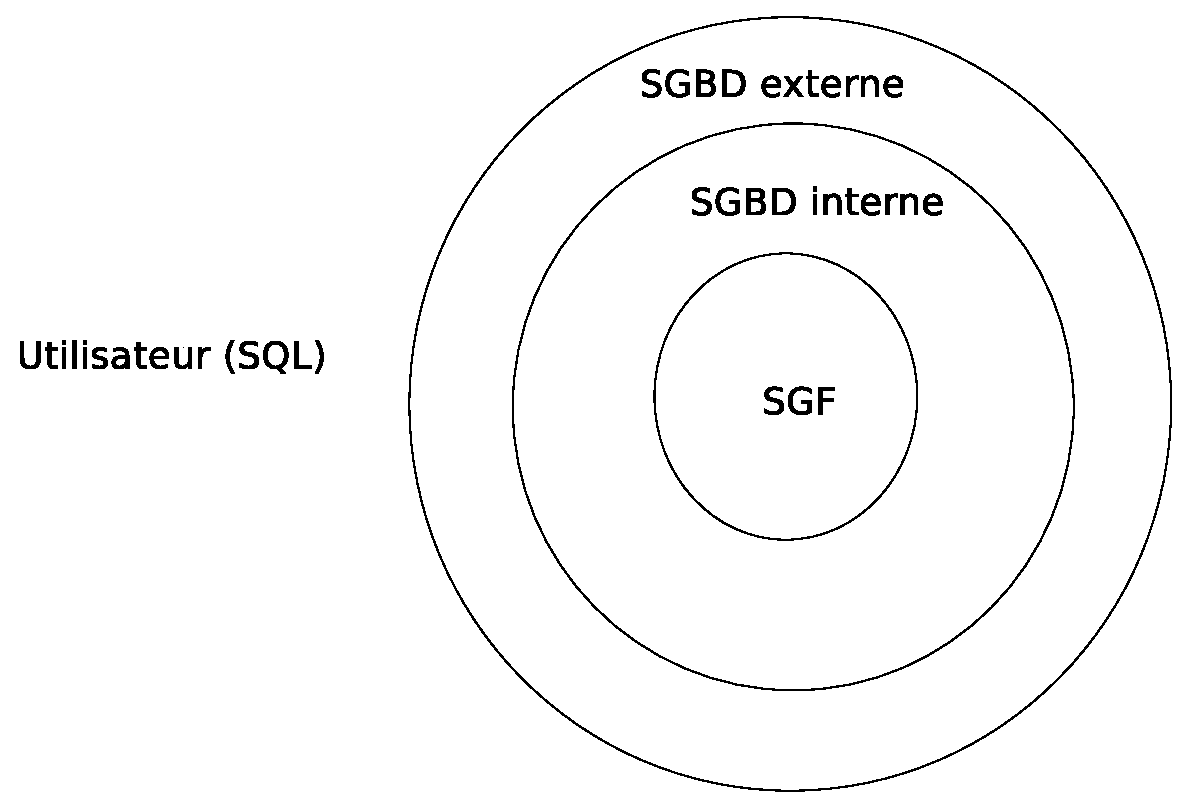
\includegraphics[width=10cm]{sgbd.eps}
		\caption{Système de Gestion de Base de Données}
	\end{figure}
	\begin{remarque}
		Le SGBD est un écran entre les usagers et les mémoires secondaires.\\ ~
	\end{remarque}
	
	Cet ensemble de programmes permet:
	\begin{itemize}
		\item La description des données
		\item L'accès aux données
		\item La mise à jour des données (insertions, modifications, destructions)
		\item La réalisation d'associations entre les données
		\item Le maintient de l'intégrité
		\item La sécurité d'exploitation
	\end{itemize}
	\section{Principale fonction d'un SGBD}
	\subsection{Fonction de description -- Description des données (LDD)}
	On doit pouvoir définir les entités se rapportant à un monde réel bien précis, préciser les attributs et les liaisons entre les entités. Le LDD
	est un outil à la disposition de l'administrateur.

	\subsection{Fonction de Manipulation -- Manipulation des données (LMD)}
	La structure de la \bd{} étant décrite : 
	\begin{itemize}
		\item Stocker / Changer les données
		\item Accéder aux enregistrements pour les mettre à jour
		\item Interroger la \bd{}
	\end{itemize}

	\subsection{Autres fonctions}
	Sécurité, intégrité, \ldots

	\section{Types d'utilisateurs d'un SGBD}
	Différents rôles que doivent jouer une personne ou un groupe de personnes pour concevoir, créer, mettre en œuvre et exploiter une \bd{} :
	\begin{description}
		\item[Administrateur]~
			\begin{itemize}
				\item Description formelle de la \bd
				\item Création des schémas externes pour les applications
				\item Définition des droits d'accès
				\item Spécifier les organisations physiques et méthodes d'accès utilisées dans l'optique de garantir les meilleures performances
				\item Définir les procédures de sécurité
			\end{itemize}
		\item[Administrateur d'application] Il est chargé de décrire la portion de la base de données concernée par une application. 
		\item[Utilisateur] 
	\end{description}

		\chapter{L'algèbre relationnelle}
		\section{Les opérations ensemblistes}
		Ce sont les opérations qui sont directement issues de la théorie des ensembles.
		\subsection{Union}
		\begin{definition}
			Opération portant sur deux relations de même schéma $R_1$ et $R_2$ consistant à construire une relation $R_3$ de même schéma et ayant
			pour tuples ceux appartenant à $R_1$, $R_2$ ou aux deux relations.
		\end{definition}
		\begin{notation}
			$R_3 = Union(R_1, R_2)$
		\end{notation}
		\begin{exemple}
			\begin{table}[H]
			\centering
			\begin{tabular}{c|c|c|c}
				\textbf{Cru} & \textbf{Millésime} & \textbf{Région} & \textbf{Couleur}\\
				\hline
				Chablis & 2008 & Bourgogne & Blanc\\
				Tavel & 2010 & Rhône & Rosé\\
			\end{tabular}
			\caption{$Vins_1$}
		\end{table}
		\begin{table}[H]
			\centering
			\begin{tabular}{c|c|c|c}
				\textbf{Cru} & \textbf{Millésime} & \textbf{Région} & \textbf{Couleur}\\
				\hline
				Lirac & 2009 & Rhône & Rouge \\
				Tavel & 2010 & Rhône & Rosé\\
			\end{tabular}
			\caption{$Vins_2$}
		\end{table}
		$$Vins_3 = Union(Vins_1, Vins_2)$$
		\begin{table}[H]
			\centering
			\begin{tabular}{c|c|c|c}
				\textbf{Cru} & \textbf{Millésime} & \textbf{Région} & \textbf{Couleur}\\
				\hline
				Chablis & 2008 & Bourgogne & Blanc\\
				Tavel & 2010 & Rhône & Rosé\\
				Lirac & 2009 & Rhône & Rouge \\
			\end{tabular}
			\caption{$Vins_3$}
		\end{table}
		\end{exemple}
		\subsection{Différence}
		\begin{definition}
			Opération portant sur deux relations de même schéma $R_1$ et $R_2$ consistant à construire une relation $R_3$ de même schéma ayant pour
			tuples ceux appartenant à $R_1$ et n'appartenant pas à $R_2$.
		\end{definition}

		\begin{notation}
			$R = difference(R_1,R_2)$
		\end{notation}
		\begin{exemple}
			\begin{table}[H]
			\centering
			\begin{tabular}{c|c|c|c}
				\textbf{Cru} & \textbf{Millésime} & \textbf{Région} & \textbf{Couleur}\\
				\hline
				Chablis & 2008 & Bourgogne & Blanc\\
				Tavel & 2010 & Rhône & Rosé\\
			\end{tabular}
			\caption{$Vins_1$}
		\end{table}
		\begin{table}[H]
			\centering
			\begin{tabular}{c|c|c|c}
				\textbf{Cru} & \textbf{Millésime} & \textbf{Région} & \textbf{Couleur}\\
				\hline
				Lirac & 2009 & Rhône & Rouge \\
				Tavel & 2010 & Rhône & Rosé\\
			\end{tabular}
			\caption{$Vins_2$}
		\end{table}
		$$Vins_3 = difference(Vins_1, Vins_2)$$
		\begin{table}[H]
			\centering
			\begin{tabular}{c|c|c|c}
				\textbf{Cru} & \textbf{Millésime} & \textbf{Région} & \textbf{Couleur}\\
				\hline
				Chablis & 2008 & Bourgogne & Blanc
			\end{tabular}
			\caption{$Vins_3$}
		\end{table}
		\end{exemple}
		\subsection{Produit}
		\begin{definition}
			Opération portant sur deux relations $R_1$ et $R_2$ consistant à construire une relation $R_3$ ayant pour schéma la concaténation
			de ceux de $R_1$ et $R_2$ et pour tuples les combinaisons des tuples de $R_1$ et $R_2$.
		\end{definition}
		\begin{notation}
			$R_3 =  pc(R_1, R_2)$
		\end{notation}
		\begin{exemple}
			\begin{table}[H]
			\centering
			\begin{tabular}{c|c|c|c}
				\textbf{Cru} & \textbf{Millésime} & \textbf{Région} & \textbf{Couleur}\\
				\hline
				Chablis & 2008 & Bourgogne & Blanc\\
				Tavel & 2010 & Rhône & Rosé\\
			\end{tabular}
			\caption{$Vins_3$}
		\end{table}
		\begin{table}[H]
			\centering
			\begin{tabular}{c|c|c|c}
				\textbf{Cru} & \textbf{Millésime} & \textbf{Région} & \textbf{Couleur}\\
				\hline
				Lirac & 2009 & Rhône & Rouge \\
				Tavel & 2010 & Rhône & Rosé\\
			\end{tabular}
			\caption{$Vins_2$}
		\end{table}
		$$Vins_6 = produit(Vins_1, Vins_2)$$
		\begin{table}[H]
			\centering
			\begin{tabular}{c|c|c|c}
				\textbf{Cru} & \textbf{Millésime} & \textbf{Région} & \textbf{Couleur}\\
				\hline
				Chablis & 2008 & Bourgogne & Blanc\\
				Tavel & 2010 & Rhône & Rosé\\
				Lirac & 2009 & Rhône & Rouge \\
				Tavel & 2010 & Rhône & Rosé\\
			\end{tabular}
			\caption{$Vins_6$}
		\end{table}
		\end{exemple}
		\section{Les opérations spécifiques}
		\subsection{Projection}
		\begin{definition}
			Opération sur une relation $R_1$ consistant à construire une relation $R_2$ en enlevant de $R_1$ tous les attributs non mentionnés en
			opérande.
		\end{definition}
		\begin{notation}
			$R_2 = \Pi_{attr_1, attr_2, \ldots, attr_n}(R_1)$
		\end{notation}
		\begin{exemple}
		\begin{table}[H]
			\centering
			$vins_7 = \Pi_{cru, region}(vins_6)$\\
			\begin{tabular}{c|c|c|c}
				\textbf{Cru} & \textbf{Région} \\
				\hline
				Chablis &Bourgogne \\
				Tavel & Rhône \\
				Lirac & Rhône \\
				Tavel & Rhône \\
			\end{tabular}
			\caption{$Vins_7$}
		\end{table}
	\end{exemple}

	\subsection{Restriction}
	\begin{definition}
	Opération sur une relation $R_1$ produisant une relation $R_2$ de même schéma mais comportant uniquement les tuples vérifiant la
	condition booléenne précisée en argument.
	\end{definition}
	\begin{notation}
		$R_2 = \sigma_{condition}(R_1)$
	\end{notation}
	\begin{exemple}
		$Vins_8 = \sigma_{region='Rhone'}(vins_6)$
		\begin{table}[H]
			\centering
			\begin{tabular}{c|c|c|c}
				\textbf{Cru} & \textbf{Millésime} & \textbf{Région} & \textbf{Couleur}\\
				\hline
				Tavel & 2010 & Rhône & Rosé\\
				Lirac & 2009 & Rhône & Rouge \\
			\end{tabular}
			\caption{$Vins_8$}
		\end{table}
	\end{exemple}

	\section{Les opérations dérivées}
	\subsection{Jointure}
	\begin{definition}
		Opération consistant à rapprocher les tuples de deux relations $R_1$ et $R_2$ afin de former une relation $R_3$ dont les attributs
		sont l'union de attributs de $R_1$ et $R_2$ et un tuple de $R_2$ vérifiant la condition précisée en argument.
	\end{definition}
	\begin{notation}
		$R_3 = join(R_1, R_2, cond)$
	\end{notation}
	\begin{exemple}
		$Vins_{10} = join(Vins_7, Vins_9, vins_7, cru=vins9.cru)$
		\begin{table}[H]
			\centering
			\begin{tabular}{c|c|c|c}
				\textbf{Cru} & \textbf{Millésime} & \textbf{Région} & \textbf{Couleur}\\
				\hline
				Chablis & 2008 & Bourgogne & Blanc\\
				Tavel & 2010 & Rhône & Rosé\\
			\end{tabular}
			\caption{$Vins_9$}
		\end{table}
	\end{exemple}

		L'opération de jointure est dérivée de l'opération de multiplication suivie d'une restriction: $join(R_1,R_2,cond) = \sigma_{cond}(pc(R_1,R_2))$

	\subsection{Intersection}
	\begin{definition}
		Opération portant sur deux relations $R_1$ et $R_2$ de même schéma consistant à construire une relation $R_3$ de même schéma ayant pour tuples
		ceux appartenant à $R_1$ et appartenant à $R_2$.
	\end{definition}
	\begin{notation}
		$R_3 = intersect(R_1, R_2)$
	\end{notation}

	L'opération d'intersection est dérivée de deux différences : \\$intersect(R_1, R_2) = difference(R_1, difference(R_1, R_2))$.

	\subsection{Division}
	\begin{definition}
		\begin{eqnarray*}
		Q = D/d = \{ <a_1,a_2,\cdots,a_p>/\forall <a_p1,ap_2,\cdots,a_n>\in d\\
		<a_1,a_2, \cdots, a_p, a_{p+1}, a_{p+2}\cdots,a_n>\in D\}&
		\end{eqnarray*}
	\end{definition}

	\begin{notation}
		
	\end{notation}

	\begin{exemple}
			\begin{table}[H]
			\centering
			\begin{tabular}{c|c}
				\textbf{NumC} & \textbf{nom}\\
				\hline
				1 & bdd\\
				2 & Archi\\
				2 & Graphe
			\end{tabular}
			\caption{$cours$}
		\end{table}
			\begin{table}[H]
			\centering
			\begin{tabular}{c|c}
				\textbf{numC} & \textbf{numE}\\
				\hline
				1&1\\
				2&1\\
				3&1\\
				1&2\\
				3&2
			\end{tabular}
			\caption{$suit$}
		\end{table}
		$$T = suit/ \Pi_{numC}(cours)$$
		\begin{table}[H]
			\centering
			\begin{tabular}{c}
				\textbf{numE}\\
				\hline
				1
			\end{tabular}
			\caption{$T$}
		\end{table}

		<< Quels sont les numéros d'étudiants qui suivent tous les cours ? >> 
	\end{exemple}

	\section{Expression de l'algèbre relationnelle}
	A partir de l'algèbre relationnelle il est possible de composer un langage algébrique.
	\subsection{Opérateur algébriques}
	Comment obtenir les couleurs de vins de cru Morgon ou Volnay ? 	

	Deux solutions sont possibles : 
	\subsubsection{Opérateur algébriques}
	\begin{eqnarray*}
		T_1 &=& \sigma_{cru='morgon'}(vins)\\
		T_2 &=&  \sigma_{cru='volnay'}(vins)\\
		T_3 &=& union(T_1, T_2)\\
		resultat &=& \Pi_{couleur}(T3)\\
	\end{eqnarray*}

	\subsubsection{Langage algébrique}
	Une autre solution, plus performante permettant de ne pas utiliser de variables temporaires en utilisant le langage algébrique : 
	\begin{eqnarray*}
		\Pi_{couleur}(union(\sigma_{cru='morgon'}(vins), \sigma_{cru='volvay'}(vins))
	\end{eqnarray*}

	\subsubsection{Arbre algébrique}
	celui-ci peut aussi être représentée sous forme d'un arbre relationnel. Les n\oe{}ud correspondent au représentation graphiques des opérations et
	les arcs aux flots de données entre les opérations.
	\begin{figure}[H]
		\centering
		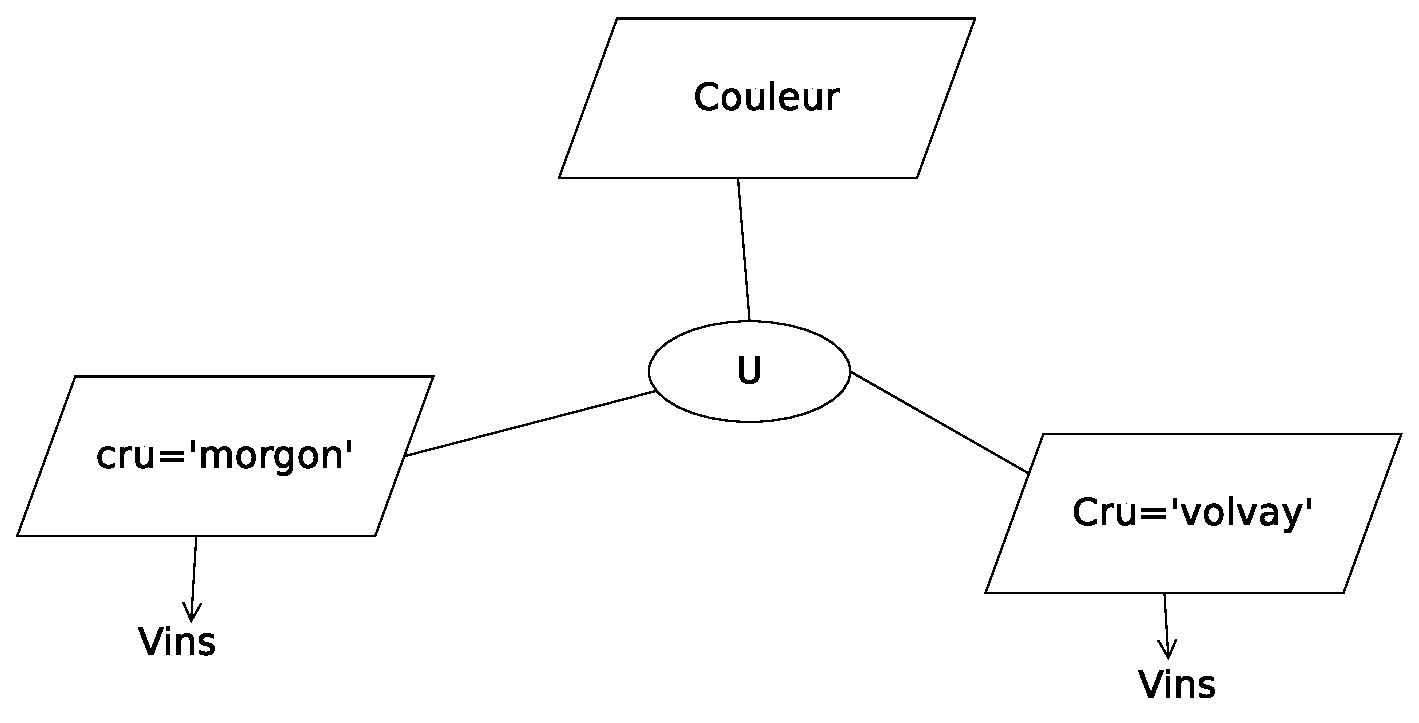
\includegraphics[width=15cm]{arbreRelationnel.eps}
		\caption{Arbre relationnel}
	\end{figure}

\chapter{Dépendances fonctionnelles}
	\section{Problèmes posés par une mauvaise perception du réel}
		\begin{table}[H]
			\begin{tabular}{cccccccccc}
				\textbf{numIm} & \textbf{Marque} & \textbf{Type} & \textbf{Puissce} & \textbf{Couleur} & \textbf{numSecu} & \textbf{nom} & \textbf{prenom} &
				\textbf{date}  & \textbf{prix}\\
				\hline
				61A3631 &Renaut & clio & 4 & Rouge & 1 & Dupont & Pierre & 10.2.13 & 10500\\
				80XA631 &Renaut & clio & 4 & bleue & 1 & Dupont & Pierre & 11.6.13 & 11600\\
				31AA31 & Citroëne & C5 & 9 & bleue & 2 & Martin & Jacques & 22.07.13 & 22000\\
				12X531 & Citroëne & C3 & 4 & verte & 2 & Martin & Jacques & 13.09.13 & 9800\\
			\end{tabular}
			\caption{Relation propriétaire}
		\end{table}

		La relation propriétaires souffre de plusieurs anomalies : 
		\begin{enumerate}
			\item \textbf{Données redondantes} Risque d'incohérence, par exemple si Jacques Martin veut changer de nom, il faudra changer tous les tuples
			\item Il est nécessaire d'autoriser les valeurs \texttt{NULL} afin de pouvoir conserver des voitures sans propriétaires ou des personnes ne
				possédant pas de voitures.
			\item \textbf{Risque de perte de données} la suppression d'un tuple peut entrainer la perte d'un type de voiture ou d'un propriétaire.
		\end{enumerate}

		\section{Approche par décomposition}
		L'approche par décomposition, pour concevoir des schémas relationnels tend à partir d'une relation universelle à découper cette relation en
		sous relation qui ne souffriraient pas des anomalies précédentes.

		\begin{definition}
			La décomposition est le remplacement d'une relation $R(A_1,A_2,\cdots,A_n)$ par une cllection de relations $R_1,R_2,\cdots R_m$ obtenus par
			des projections de R et tels que la relation résultat des jointures $R_1\bowtie R_2\bowtie \cdots \bowtie R_m$ ait le même schéma que R.
		\end{definition}

		\begin{exemple}
		\begin{table}[H]
			\centering
				\begin{tabular}{cccccccccc}
					\textbf{numIm} & \textbf{Marque} & \textbf{Type} & \textbf{Puissce} & \textbf{Couleur} \\
					\hline
					872RH75 & Renaut & Clio & 6 & Verte\\ 
					31AA31 & Renaut & Clio & 6 & Rouge\\
				\end{tabular}
				\caption{Relation Voiture}
				\begin{tabular}{ccc}
					\textbf{numIm} & \textbf{Type} & \textbf{Couleur} \\
					\hline
					872RH75 & Clio & Verte\\ 
					31AA31 & Clio & Rouge\\
				\end{tabular}\hspace{20px}
				\begin{tabular}{ccc}
					\textbf{type} & \textbf{Marque} & \textbf{Puissance}\\
					\hline
					Clio & Renault & 6\\
				\end{tabular}
				\caption{Décomposition 1}
				$T_1 = R_1 \bowtie R_2$\\
				\begin{tabular}{cc}
					\textbf{numIm} & \textbf{Type} \\
					872RH75 & Clio\\ 
					31AA31 & Clio\\
				\end{tabular}
				\begin{tabular}{ccc}
					\textbf{type} & \textbf{Marque}\\
					Clio & Renault\\
				\end{tabular} 
				\begin{tabular}{ccc}
					\textbf{type} & \textbf{Puissance} & \textbf{Couleur}\\
					Clio & 6 & Verte\\
					Clio & 6 & Rouge\\
				\end{tabular} \\
				$T_2 = \bowtie v_1 \bowtie v_2 \bowtie v_3$\\
				\begin{tabular}{cccccccccc}
					\textbf{numIm} & \textbf{Marque} & \textbf{Type} & \textbf{Puissce} & \textbf{Couleur} \\
					\hline
					872RH75 & Renaut & Clio & 6 & Verte \\ 
					31AA31 & Renaut & Clio & 6 & Rouge\\
				\end{tabular}
				\caption{Décomposition 2}
			\end{table}
			Perte d'information sur la couleur.
		\end{exemple}
		La décomposition 1 permet de retrouver l'information par jointure alors que la décomposition 2 ne permet pas de retrouver la couleur d'une
		voiture.

		\begin{definition}
			La décomposition sans perte d'informations, ou spi est la décomposition d'une relation R en $R_1,R_2,\cdots,R_n$ par toute extension de R,
			on ait $R=_1\bowtie R_2\bowtie \ldots \bowtie R_4$.
		\end{definition}
		
		\section{Notion de dépendances fonctionnelles}
		La notion de dépendances fonctionnelles (df) permet de caractériser les relations qui peuvent être décomposée sans perte d'information.

		\begin{definition}
			\textbf{Dépendance fonctionnelle}: soit $R(A_1,R_2,\cdots,R_n)$ un schéma de relation et $X$ et $Y$ des sous-enembles de
			$\{A_1,A_2,\cdots,A_n\}$. On dit que $X\rightarrow Y$ ($x$ détermine $Y$) si pour tout extensions $r$ de $R$, pour tout tuple $t_1$ et
			$t_2$ de $r$ on a $\Pi_X(t_1) = \Pi_X(t_2) \Rightarrow \Pi_Y(t_1) = \Pi_Y(t_2)$
		\end{definition}
\begin{remarque}
	$X\rightarrow$Y si étant donné une valeur de $X$, il lui correspond une valeur unique de $Y$
\end{remarque}
		\begin{exemple}
			\begin{tabular}{cc}
				numIm $\rightarrow$ Type & Type $\rightarrow$ Puisance\\
				numIn $\rightarrow$ Couleur & Type $\rightarrow$ marque\\
				Type,Marque $\rightarrow $puissance
			\end{tabular}\\
			Par contre on a pas Puissance $\not\rightarrow$ type.

			Il est possible de visualiser cet ensemble de df par un graphe appelé graphe de dépendance fonctionnelle.
		\end{exemple}

		\subsection{Théorèmes}
		\subsubsection{Axiomes d'Amstrong}
		\begin{description}
			\item[Réfléxivité] $Y \subseteq X \Rightarrow X \rightarrow Y$ Tout ensemble d'attribut détermine les même où une partie de lui même
			\item[Augmentation] $X\rightarrow Y \Rightarrow X,Z \rightarrow Y,Z$ si $X\rightarrow Y$ les deux ensembles d'attributs peuvent être
				enrichis par une troisième
			\item[Transitivité: $X\rightarrow Y$ et $Y \rightarrow Z \Rightarrow X\rightarrow Z$] Cette règle provient du fait que le composé de deux
				fonctions dont l'image de l'une et le domaine de l'autre est une fonction.
		\end{description}

		\subsubsection{Règles déduites}
		Plusieurs règles se déduisent de ces axiomes : 
		\begin{description}
			\item[Union] $X\rightarrow Y$ et $X\rightarrow Z \Rightarrow X \rightarrow y,Z$
			\item[Pseudo transitivité] X$\rightarrow Y$ et $W,Y \rightarrow Z \Rightarrow W,X \rightarrow Z$ 
			\item[Décomposition] $X\rightarrow Y$ et $Z\subseteq  \Rightarrow X\rightarrow Z$ 
		\end{description}

		\begin{definition}
			Une dépendance fonctionnelle élémentaire est une dépendance de a forme $X \rightarrow A$, ou $A$ est un attribut unique $\not\in X$ et où
			$\not\exists X \subset X$ tel que $X \rightarrow A$.
		\end{definition}
		\begin{exemple}
			type $\rightarrow$ puissance n'est pas élémentaire
		\end{exemple}
		\begin{remarque}
			La seule règle d'inférance qui s'applique au dépendances fonctionnelles et la transitivté.~\\
		\end{remarque}

		\begin{definition}
			Une clé est un sous ensemble $X$ des attributs d'une relation $R(A_1,A_2,\cdots,A_n)$
			tel que $X\rightarrow A_1,A_2,\cdots,A_n$ et $\not\exists Y \subset Y$ tel que $Y\rightarrow A_1,A_2,\cdots,A_n$.
		\end{definition}
		
		\begin{definition}
			La fermeture transitive est un ensemble de dépendances fonctionnelles considéré enrichi de toutes les dépendances fonctionnelles déduites
			par transitivité.

			Notation: La fermeture transitive de F est noté $F^+$
		\end{definition}

		\begin{definition}
			2 ensembles $F_1$ et $F_2$ sont équivalent ssi $F_1^+ = F_2^+$	
		\end{definition}

		\begin{definition}
			La convention minimale est un ensemble F de dfe associé à un ensemble d'attributs vérfiant les propriétés suivantes : 
			\begin{enumerate}
				\item Aucune df n'est redondante $\forall f \in F$, $F.f$ n'est pas équivalent à $F$.
				\item Toute dfe est dans $F^+$
			\end{enumerate}
		\end{definition}

		\begin{proposition}
			Si une relation $R(X,Y,Z)$ possède une dépendance $X\rightarrow Y$ alors $R$ est décomposable sans perte d'information en $R_1(X,Y)$ et
			$R_2(X,Z)$.
		\end{proposition}
		\section{Formes Normales (NF)}
		\begin{definition}
			Une relation est en première forme normale si tout attriut contient une valeur atomique, éviter le domaine composé de plusieurs valeurs	
		\end{definition}
		\begin{definition}
			Une relation R est en 2eme forme normale si : 
			\begin{itemize}
				\item Elle est en 1NF
				\item Tout attribut n'appartenant pas à une clé ne dépend pas d'une partie de la clé
			\end{itemize}
		\end{definition}
		\begin{exemple}
			Fournisseur(\underline{nom, article}, adresse, prix)\\
			d1: nom,article $\rightarrow$ prix\\
			d2: nom $\rightarrow$ adresse

			Cette relation n'est pas en 2NF à cause de d2
		\end{exemple}
		\begin{definition}
			Une relation est en 3e forme normal si et seulement si : 
			\begin{itemize}
				\item Elle est en 2NF
				\item Tout attribut n'appartenant pas à une clé ne dépend pas d'un attribut n'appartenant pas à un clé.
			\end{itemize}
		\end{definition}
		\begin{exemple}
			voitures(\underline{numIm, type}, marque)\\
			d1: numIm $\rightarrow$ type\\
			d2: type $\rightarrow$ marque

			Voiture n'est pas en 3NF à cause de d2.
		\end{exemple}

		\begin{definition}
			Une relation est en 3NF BKC, Bayo-Codd Kent, si et seulement si les seules différences sont celles dans lesquelles une clé détermine un
			attribut.
		\end{definition}

		\section{Algorithme de décomposition 3NF}
		Pour toute relation, il existe au moins une décomposition en 3NF préservant les dépendances fonctionnelles sans perte d'information. Le but d'un
		algorithme de décomposition en 3NF est de convertir un schéma de relation qui n'est pas 3NF en un ensemble de schémas 3NF.

		Le principe de l'algorithme consiste à appliquer les règle e décomposition suivantes tel que les schémas ne sont pas 3NF:
		\begin{description}
			\item[Schéma non 2NF] R(k1, k2, x, y); La relation doit être décomposée en R1(\underline{k2}, X) et R2(\underline{k1,k2}, Y)
			\item[Schéma non 3NF] R(k,x,y,z), la relation doit être décomposée en R1(\underline{X},Z) et R2(\underline{k},x,y)
		\end{description}
		\begin{itemize}
			\item Schéma non 2NF
		\end{itemize}
		\section{Propriétés d'une décomposition en 3NF}
		Les dépendances fonctionnelles des règles indépendants du temps qui doivent vérifier les attributs, il est nécessaire qu'une décomposition
		préserve les règles

		\begin{definition}
			Une décomposition $\{R_1,R_2,\cdots,R_n\}$ d'une relation R tel que la fermeture transitive de la df de R est le même que l'union des
			dépendances fonctionnelles de $\{R_1,R_2,\cdots,R_n\}$.
		\end{definition}

		Dans toute relation, il existe au moins une décomposition en 3NF préservant les dépendances fonctionnelles sans perte d'information. Le but
		d'un algorithme de décomposition en 3NF est de convertir un schéma de relation qui n'est pas 3NF.

	\appendix
	\chapter{Exercices}
\section{Algèbres relationnel}
\subsection{Opérateurs algébriques}
\texttt{ vins(numv, cru, mill, region, degré) } \\
\texttt{ buveurs(nums, nom, prenom, ville) } \\	
\texttt{ abus(nomv, nomb, date, quantite, place) } \\

	
\begin{attention}
Avec les opérateurs algébriques et uniquement les opérateurs de base. 
\end{attention}

\subsubsection{ Donner le degré des vins de cru Morgon et Millésime 2001 }
\begin{eqnarray*}
	T_1 &=& \sigma_{cru='morgon'~and~mill=2001}(vins)\\
	T_2 &=& \pi_{degré}(T_2)
\end{eqnarray*}
\subsubsection{Numéro des buveurs de Chenas}
\begin{eqnarray*}
	T_1 &=& \sigma_{cru='chenas'}\\
	T_2 &=&  pc(T_1, abus)\\
	T_3 &=& \sigma_{T_1.numV = abus.numV}(T_2)\\
	Res &=& \Pi_{numB}(T3)
\end{eqnarray*}

\subsubsection{Nom et prénom des buveurs de chénon et de Tariquet}
\remarque{Autorisation d'utiliser le join\\~}

\begin{eqnarray*}
	T_1 &=&  \sigma_{cru='chenon' ou cru='tariquet'}(vins)\
	T_2&=&   join(T_1, abus, T_2.numV= abus.numV)\\
	T_3 &=& join(T_2, buveurs, T_2.numB=buveurs.numB)\\
	Res &=& \Pi_{nom, prenom}(T_3)
\end{eqnarray*}

\end{document}
